\documentclass[11pt]{article}
% Adapted from an original template by Hlyni Arnórssyni,
% Reykjavik University, Iceland

% ------------------------------ PAGE SETTINGS ------------------------------
\usepackage{geometry}

\geometry{
    paper=a4paper,
    top=2.5cm,
    bottom=2.5cm,
    left=2.5cm,
    right=2.4cm,
    headheight=0.75cm,
    footskip=1.5cm,
    headsep=0.75cm
}

% ------------------------------ BASIC PACKAGES ------------------------------
\usepackage{blindtext}

% Character encoding
\usepackage[T1]{fontenc}
\usepackage[utf8]{inputenc}

% Mathematics
\usepackage{amsmath, amsfonts, amsthm, amssymb}
\usepackage{braket, nicefrac}

% SI units
\usepackage{siunitx}

% Lists / columns
\usepackage{enumitem, multicol}

% ------------------------------ FIGURES ------------------------------
\usepackage{graphicx}
\usepackage{float}
\usepackage{keystroke}
\usepackage{pgfplots}
\usepgfplotslibrary{units}
\pgfplotsset{compat=1.16}

% Search these locations automatically for figures
\graphicspath{{fig/}{graphics/}{Graphics/}{./}}

% ------------------------------ TABLES ------------------------------
\usepackage{tabularx}
\usepackage{array}
\usepackage[table]{xcolor}

% ------------------------------ TYPOGRAPHY ------------------------------
\usepackage{caption}
\usepackage{titlesec}
\usepackage{microtype}
\usepackage{csquotes}

% ------------------------------ COLORS ------------------------------
\definecolor{GWBlue}{HTML}{1E4E79}

% ------------------------------ SECTION STYLING ------------------------------
\titleformat{\section}
  {\Large\bfseries\color{GWBlue}}
  {\thesection.}
  {0.40em}
  {}

\titlespacing*{\section}
  {0pt}
  {0.70em}
  {0.28em}

% ------------------------------ CAPTION STYLING ------------------------------
\captionsetup{
    font=small,
    labelfont=bf,
    textfont=it,
    labelsep=period,
    skip=4pt
}

% ------------------------------ PARAGRAPH SPACING ------------------------------
\setlength{\parindent}{0pt}
\setlength{\parskip}{0.30em}

% ------------------------------ BIBLIOGRAPHY ------------------------------
\usepackage[
    backend=biber,
    style=authoryear,
    sorting=none,
    giveninits=true,
    maxbibnames=99,
    dashed=false
]{biblatex}

\addbibresource{references.bib}

\DeclareNameAlias{sortname}{family-given}
\DeclareNameAlias{default}{family-given}
\DeclareFieldFormat[article]{title}{#1}
\DeclareFieldFormat[misc]{title}{#1}
\renewbibmacro{in:}{}

\AtEveryBibitem{%
    \clearfield{doi}%
    \clearfield{urldate}%
}

\AtBeginBibliography{\small}
\setlength{\bibitemsep}{0.35em}

% ------------------------------ HYPERLINKS ------------------------------
\usepackage{hyperref}

\hypersetup{
    colorlinks=true,
    linkcolor=GWBlue,
    citecolor=GWBlue,
    urlcolor=GWBlue
}

\begin{document}

\begin{titlepage}
\centering
\thispagestyle{empty}

\vspace*{0.15in}


\includegraphics[
    width=0.5\textwidth
]{gwu_logo.pdf}

\vspace{0.28in}

{\large\bfseries Data Science Program\par}
{\large\bfseries Department of Data Science\par}
{\large DATS 6501 - Capstone Project - Fall 2026\par}

\vspace{0.38in}

{\Large\bfseries
Post-Training Analysis \& Novelty Detection Using\par}

\vspace{0.08in}

{\Large\bfseries
Neural Network Self-Organizing Maps (NNSOM)\par}

\vspace{0.34in}

{\large\bfseries
PHASE 1 REPORT\par}

\vspace{0.22in}

{\large\bfseries
Baseline Model Training \& Latent Feature Extraction\par}

\vspace{0.36in}

{\large\bfseries Capstone - Group 5\par}

\vspace{0.08in}

{\large\bfseries Fyrooz Khan\par}
{\large\bfseries Nazish Atta\par}

\vspace{0.30in}

{\large The George Washington University\par}
{\large Washington, DC\par}

\vspace{0.30in}

{\large\itshape Supervised by\par}
{\large\itshape Dr. Amir Jafari\par}
{\large\itshape Associate Professor of Data Science\par}

\vspace*{\fill}

\end{titlepage}

\setcounter{page}{2}

\section{Week 2 Overview}

Week 2 completed the baseline modeling stage of the capstone. The MNIST
dataset was prepared using a stratified 70/15/15 train-validation-test
split, a LeNet-5 convolutional neural network was trained and evaluated,
and 84-dimensional feature embeddings were extracted from the
penultimate \texttt{fc2} layer for later Self-Organizing Map analysis.

\section{Related Work}

Convolutional neural networks provide the supervised representation-learning
foundation for this project. LeCun et al.~\cite{lecun1998gradient} showed that
CNNs can learn effective hierarchical features for handwritten character
recognition. Our work does not propose a new classifier architecture; instead,
it treats a trained CNN as a source of latent representations whose organization
and failures can be studied after training.

Self-Organizing Maps offer a complementary way to inspect high-dimensional
structure. Kohonen's original SOM~\cite{kohonen1990som} preserves neighborhood
relationships on a low-dimensional grid, while Vesanto and
Alhoniemi~\cite{vesanto2000clustering} showed how trained SOM prototypes can
support quantitative clustering. More recent methods integrate neural
representation learning directly with SOM organization, including
SOM-VAE~\cite{fortuin2019somvae} and Deep Embedded Self-Organizing
Maps~\cite{forest2021desom}. In contrast, this capstone keeps the supervised
CNN fixed during the initial NNSOM analysis so that SOM-derived diagnostic
signals can be evaluated separately from representation learning.

A second relevant line of work concerns novelty and out-of-distribution (OOD)
detection. Maximum softmax probability provides a simple post-hoc baseline
\cite{hendrycks2017baseline}, while ODIN modifies inference using temperature
scaling and input perturbations~\cite{liang2018odin}. Lee et
al.~\cite{lee2018mahalanobis} use Mahalanobis distance in deep feature space,
Deep SVDD learns a compact one-class representation~\cite{ruff2018deep}, and
energy-based scoring provides another strong output-space OOD signal
\cite{liu2020energy}.
These studies motivate rigorous comparison because they
show that useful novelty information can appear in either classifier outputs
or latent features.

The distinguishing hypothesis of this project is therefore not that SOMs are
automatically superior to these methods. Rather, we test whether NNSOM
quantization and topology applied to fixed CNN embeddings expose structured
error regions and provide useful novelty signals. This post-training framing
connects SOM representation analysis with classifier failure geography while
keeping the contribution empirically testable against established baselines.

\section{Methodology}

\begin{table}[H]
\centering
\renewcommand{\arraystretch}{1.10}

\begin{tabular}{|p{0.42\textwidth}|p{0.48\textwidth}|}
\hline
\textbf{Item} & \textbf{Week 2 Setup} \\
\hline
Dataset & MNIST, 70,000 grayscale images ($28 \times 28$) \\
\hline
Split & 49,000 train / 10,500 validation / 10,500 test \\
\hline
Model & LeNet-5 CNN \\
\hline
Training & 20 epochs, Adam optimizer, cross-entropy loss \\
\hline
Feature layer & \texttt{fc2} penultimate layer, 84 dimensions \\
\hline
\end{tabular}
\end{table}

The best validation checkpoint was used for final test evaluation and
feature extraction. The saved \texttt{fc2} embeddings from all three
splits provide the input for NNSOM in Week 3.

\begin{figure}[H]
\centering
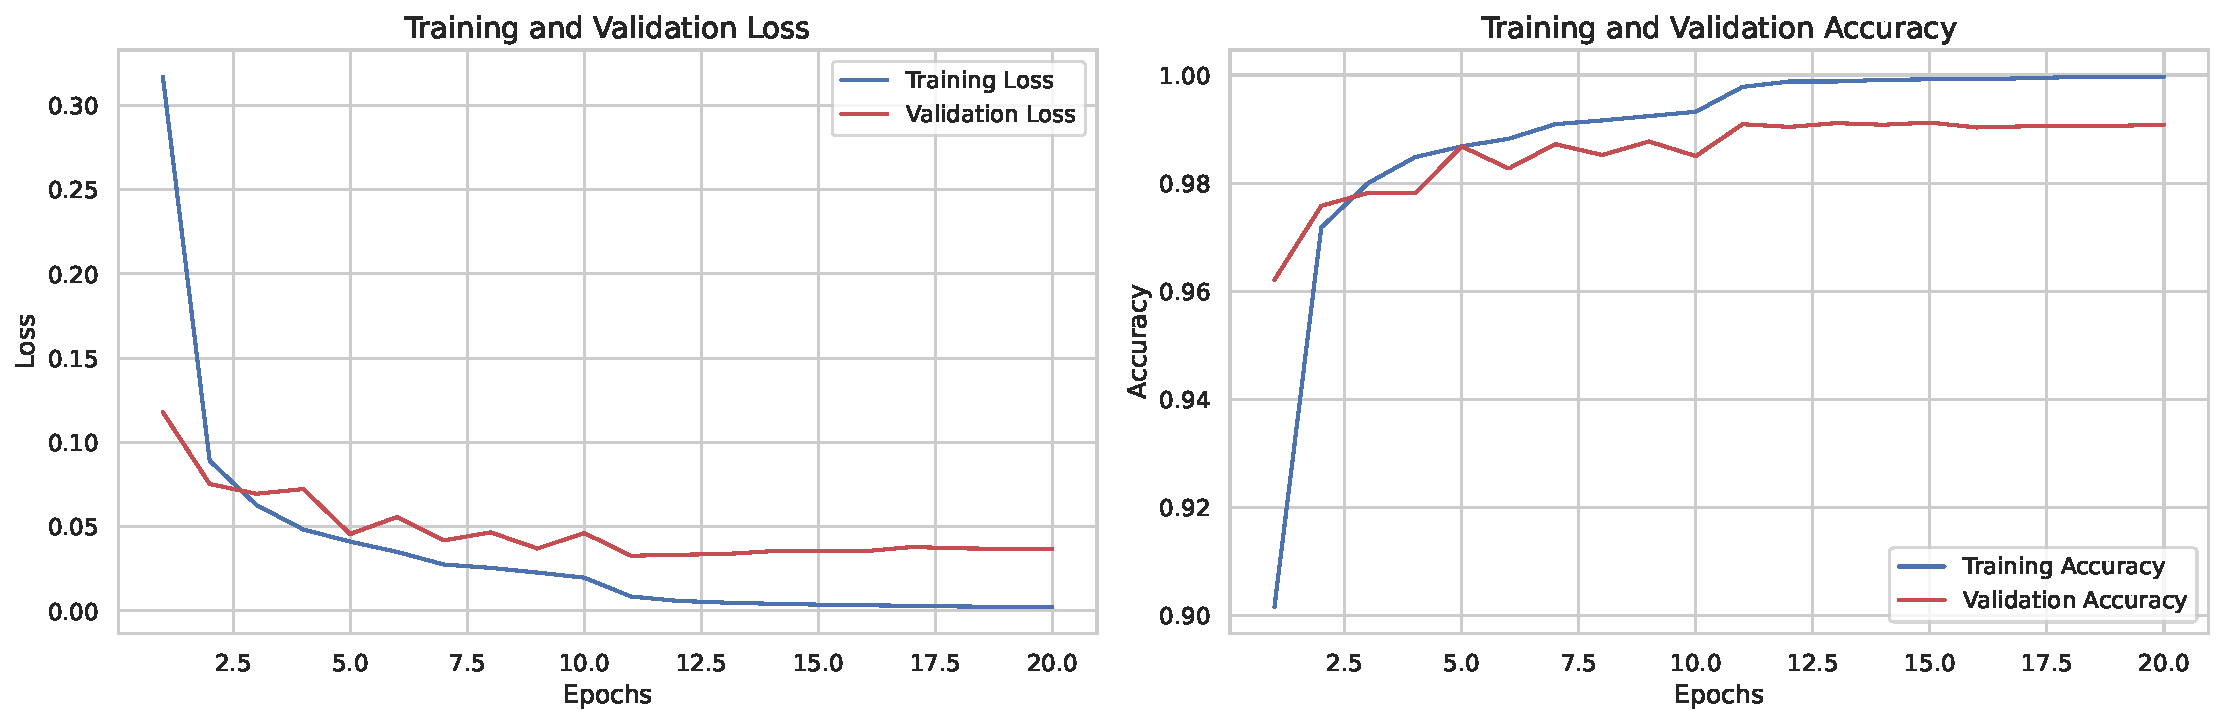
\includegraphics[
    width=0.88\textwidth,
    keepaspectratio
]{cnn_baseline/training_curves.pdf}
\caption{Training and validation loss/accuracy across 20 epochs.}
\label{fig:training-curves}
\end{figure}

\section{Results}

\begin{table}[H]
\centering
\renewcommand{\arraystretch}{1.10}

\begin{tabular}{|p{0.42\textwidth}|p{0.48\textwidth}|}
\hline
\textbf{Metric} & \textbf{Result} \\
\hline
Test accuracy & 99.18\% (10,414 / 10,500); 95\% Wilson interval 98.99\%--99.34\% \\
\hline
Macro F1-score & 0.9918 \\
\hline
Misclassified samples & 86 (0.82\%) \\
\hline
Embedding output & 84-dimensional \texttt{fc2} vectors \\
\hline
\end{tabular}
\end{table}

The baseline generalized well to the held-out test set. The 95\% Wilson
score interval for the test accuracy, 98.99\%--99.34\%, shows the
uncertainty that comes from evaluating on 10,500 images. Errors were
sparse and concentrated among a small number of class pairs; the most
frequent individual confusions included $7\rightarrow1$,
$5\rightarrow8$, and $2\rightarrow8$, with four cases each.
Digit 0 had only one misclassification.

\clearpage

\begin{figure}[H]
\centering
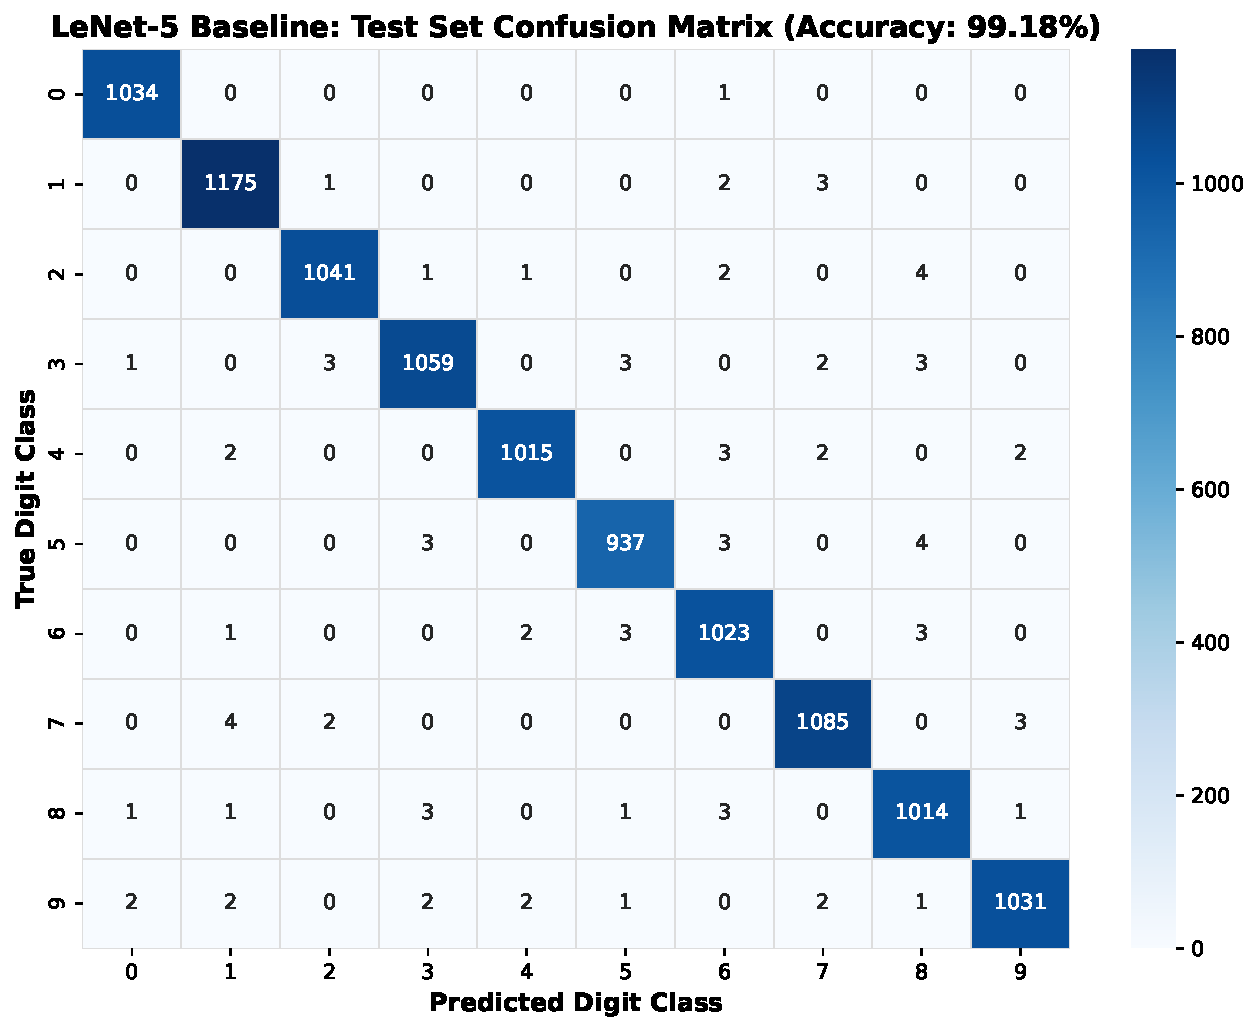
\includegraphics[
    width=0.72\textwidth,
    keepaspectratio
]{cnn_baseline/confusion_matrix.pdf}
\caption{Test-set confusion matrix. The strong diagonal indicates high class-level accuracy.}
\label{fig:confusion}
\end{figure}

\section{Latent Feature Representation}

For every sample, the 84-dimensional activation from the
\texttt{fc2} layer was extracted and saved. This representation
captures the learned features immediately before the final
classification layer and is the feature space that will be analyzed
with NNSOM.

\clearpage

\begin{figure}[H]
\centering
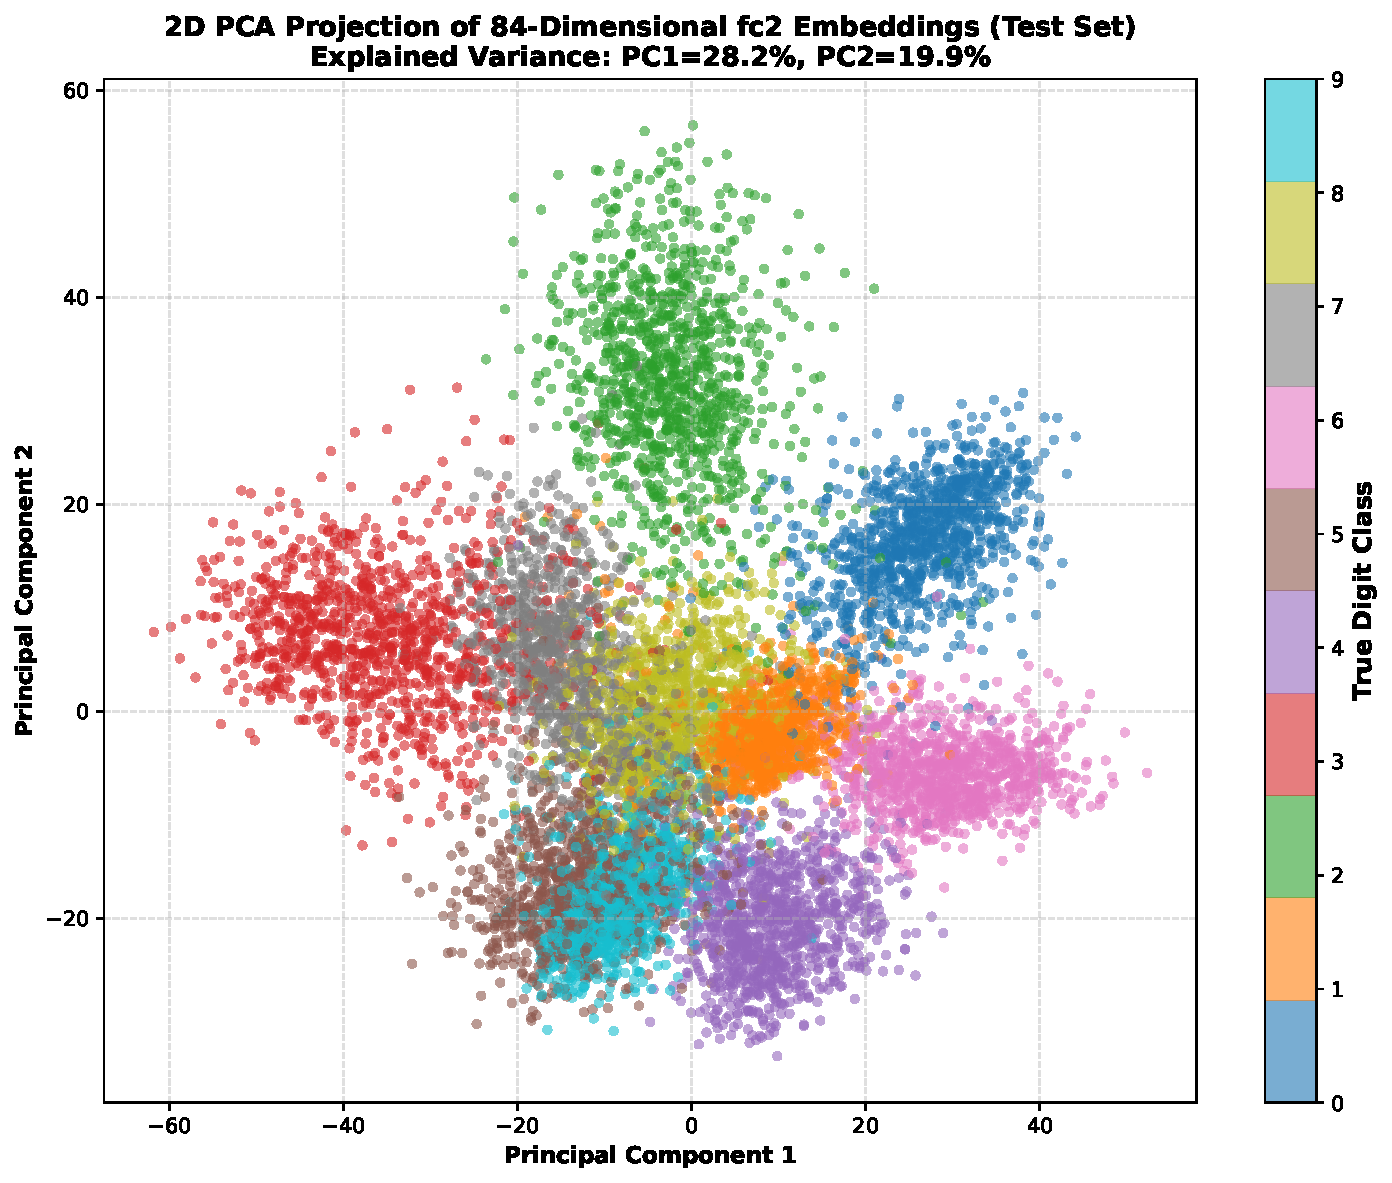
\includegraphics[
    width=0.70\textwidth,
    keepaspectratio
]{cnn_baseline/fc2_pca.pdf}
\caption{PCA projection of the 84-dimensional \texttt{fc2} test embeddings for visualization only.}
\label{fig:pca}
\end{figure}

The PCA view is only a preliminary 2D visualization; Week 3 will use
the full 84-dimensional training embeddings as the actual input to
NNSOM.

\section{Leakage Control}

The test split was kept out of every development decision:

\begin{itemize}
    \item The 70,000 images were split once, by a stratified split with a fixed
    seed (42), into 49,000 training, 10,500 validation and 10,500 test images.
    Every image has a fixed sample ID, so the three splits never overlap.

    \item Pixels were only scaled to $[0,1]$ (divided by 255). No statistic was
    computed from the data for normalization, and no augmentation was used.

    \item The model was trained on the training split only. The checkpoint was
    chosen by validation accuracy; the training settings (20 epochs, Adam,
    learning rate and schedule) were fixed in the configuration file and were
    not tuned on the test split.

    \item The test split was evaluated once, after training, for the accuracy,
    F1-score and confusion matrix reported above.

    \item Test embeddings were saved for completeness, but the SOM analysis that
    follows uses the training and validation embeddings only.
\end{itemize}

\section{Conclusion and Week 3 Transition}

Week 2 established a reproducible MNIST baseline and produced the
feature embeddings required for the next phase. In Week 3, NNSOM~\cite{jafari_nnsom} will
be configured and trained on the 49,000 training embeddings to map
samples to Best Matching Units, monitor quantization error, and
visualize class organization using SOM-based plots such as hit maps
and the U-Matrix.

\clearpage
\printbibliography[title={References}]

\end{document}